\part*{Características gerais do jogo}
\section{Apresentação do jogo}
\subsection{Objetivo do documento}
O objetivo desse documento é apresentar as características principais do jogo 7 Keys, sua história, mecânicas, a proposta de design entre outras informações importantes para o desenvolvimento do jogo.

\subsection{Objetivo do jogo}     
O principal objetivo do jogo é fugir do santório. O jogador começa na ala de celas e precisa alcançar o térreo. Para finalizar cada fase será necessário encontrar uma chave específica que abra a porta que dá acesso ao andar inferior ou à próxima ala.

\subsection{Características gerais}

O jogo terá uma movimentação semelhante a games do estilo Legend of Zelda a Link to the Past e Fatal Labirinth como principais referências e exemplos os jogos The Binding of Isaac e Metal Gear Solid IV como referência para a mecânica de stealth.

 O jogo baseia-se em dois gêneros: stealth e roguelike. Stealth é um gênero onde o jogador precisa evitar ser notado, utilizando da furtividade para evadir ou elaborar emboscadas para os antagonistas. Jogos do gênero empregam mecânicas como se esconder na sombra, em objetos do cenário, disfarces, e barulhos que podem alertar os inimigos. Roguelike é um subgênero, geralmente de jogos de RPG, que é caracterizado pela geração de mapas aleatórios durante a partida, mapas baseados em tile e permanent death.

Não haverá também coleta de moedas, diamantes ou qualquer referência a acúmulo de material destinado à compra de itens, vidas etc. Todos os itens necessários para avançar no jogo estarão dispostos nas fases.

O jogo não possuirá um contador de pontos pois foi considerado dispensável devido a mecânica do jogo.

\section{Requisitos Tecnológicos}
Para a atividade de desenvolvimento foi estabelecida a utilização das seguintes ferramentas:

\begin{enumerate}
\item Sistema Operacional: Linux Ubuntu 14.04 64-bits

Este SO foi escolhido por ser uma ferramenta open source e de utilização comum para a maioria da equipe de desenvolvimento.

\item APIs para manipulação de arquivos, áudio e gráfica: SDL2/SDL1.2

API padrão da disciplina.

\item Ferramenta de controle de versão: Git

Ferramenta padrão da disciplina.

\item Depurador: Debugger

Por ser o software padrão do Linux Ubuntu, o depurador Debugger, da suite GNU, será utilizado.

\item Editor de texto: Sublime Text 2 

O editor Sublime Text 2 está sendo utilizado, porém será decidido por um novo editor em breve.

\item Linguagem de script: Lua

Linguagem de script padrão da disciplina.

\item Linguagem de programação: C++

Esta linguagem foi escolhida por ser de compreensão comum para a maioria da equipe de desenvolvimento.

\item Compilador: g++

\end{enumerate}

\section{Front End}
Ao iniciar o jogo algumas telas são apresentadas ao jogador. Elas contém informações básicas porém importantes, como a empresa que desenvolveu o jogo e as tecnologias ligadas à ele. 

No caso do jogo proposto nesse documento, desenvolvido pela Mana Team, a primeira tela ao executar o jogo que aparece é a tela que apresenta o logo da equipe (Figura 1), que é também o mascote da empresa, o peixe boi. Em seguida vem a tela que apresenta as tecnologias utilizadas para desenvolver o jogo (Figura 2), como o GIMP, os programas da Adobe entre outros. Por fim, antes da tela do menu inicial, vemos a tela com a classificação indicativa do jogo (Figura 3). Cada tela ficará visível por 3 segundo e após esse período ocorrerá um efeito de \textit{fade out} com duração de 1 segundo seguido de um efeito de \textit{fade in} também de um segundo que introduzirá a tela seguinte. A música do menu será iniciada no instante em que a primeira tela for carregada.
\begin{figure}[h]
    \centering
    \caption{Tela com logo [provisória] da empresa}
     
\includegraphics[keepaspectratio=true,scale=0.30]{images/logoMT.png}
\end{figure}
\begin{figure} [!h]
    \centering
    \caption{Tecnologias utilizadas}
    
\includegraphics[keepaspectratio=true,scale=0.30]{images/tecnologias.png}
\end{figure}
\begin{figure}[!h]
    \centering
    \caption{Classificação Indicativa}
    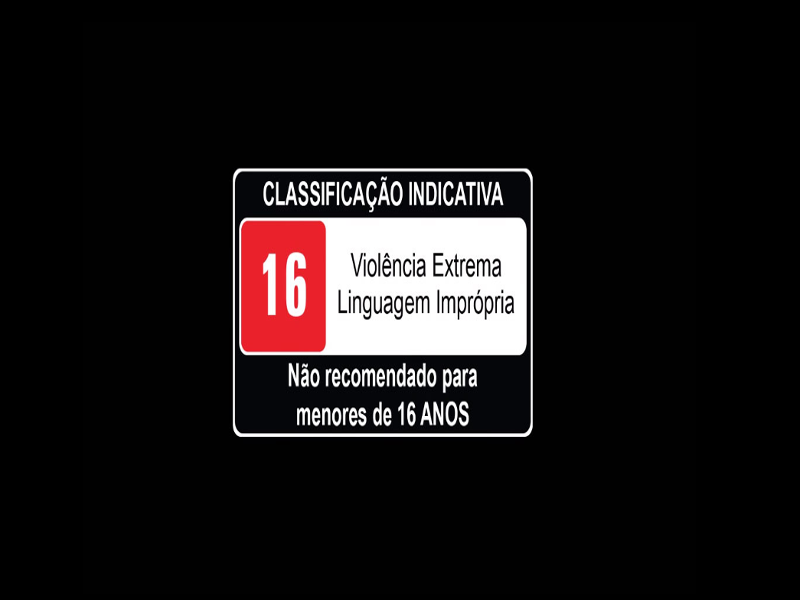
\includegraphics[keepaspectratio=true,scale=0.30]{images/classificacao_indicativa.png}
\end{figure}

\section{Telas}
Essa seção visa mostrar as telas do menu inicial do jogo e o menu de pause. Na tela de extras o jogador poderá escolher entre rever o vídeo de abertura do jogo ou ler a história completa do Edmond, para maior compreensão do jogo.

\begin{figure}[!h]
    \label{menu}
    \centering
    \caption{Menu Inicial do jogo}
    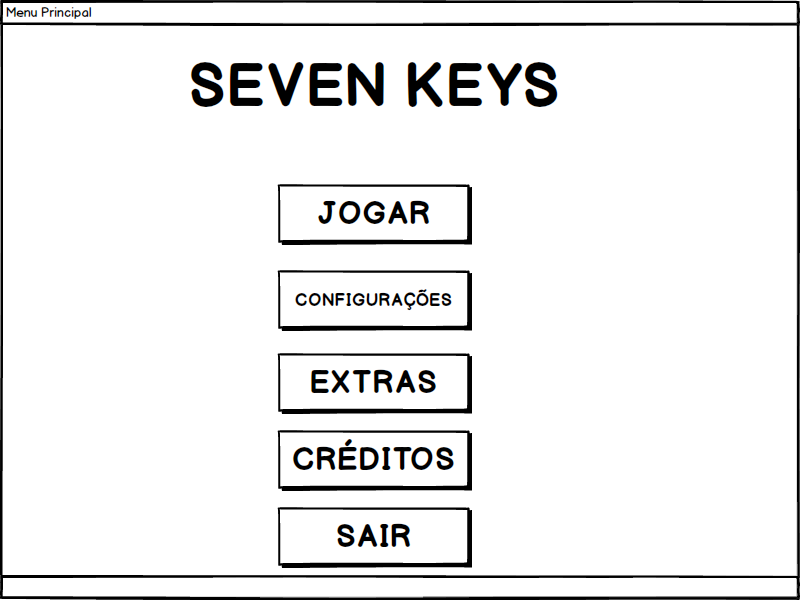
\includegraphics[keepaspectratio=true,scale=0.35]{images/MENU.png}
\end{figure}

\begin{figure}[!h]
    \label{Tfase}
    \centering
    \caption{Tela de seleção de fase}
    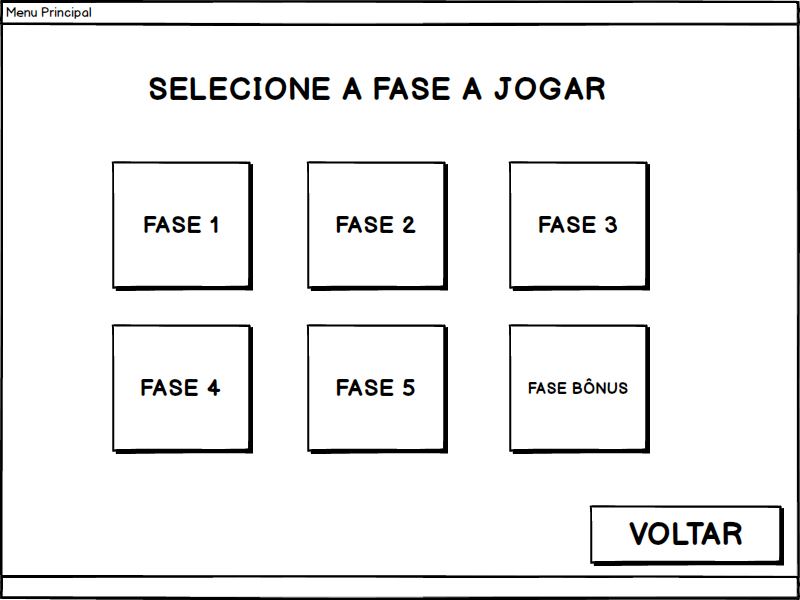
\includegraphics[keepaspectratio=true,scale=0.35]{images/JOGAR.png}
\end{figure}

\begin{figure}[!h]
    \label{Tconfig}
    \centering
    \caption{Tela de configurações}
    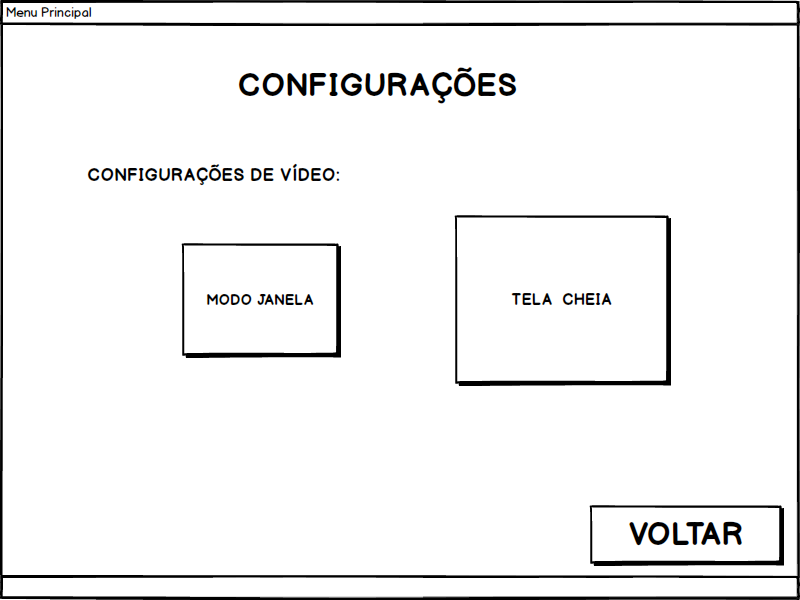
\includegraphics[keepaspectratio=true,scale=0.35]{images/CONFIG.png}
\end{figure}

\begin{figure}[!h]
    \label{Textra}
    \centering
    \caption{Tela de conteúdo extras}
    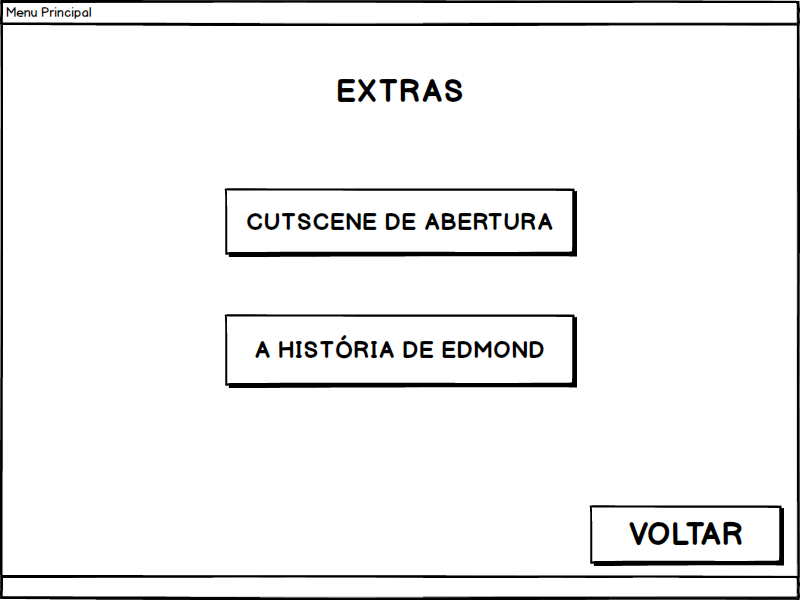
\includegraphics[keepaspectratio=true,scale=0.35]{images/EXTRAS.png}
\end{figure}

\begin{figure}[!h]
    \label{Tcred}
    \centering
    \caption{Tela de créditos}
   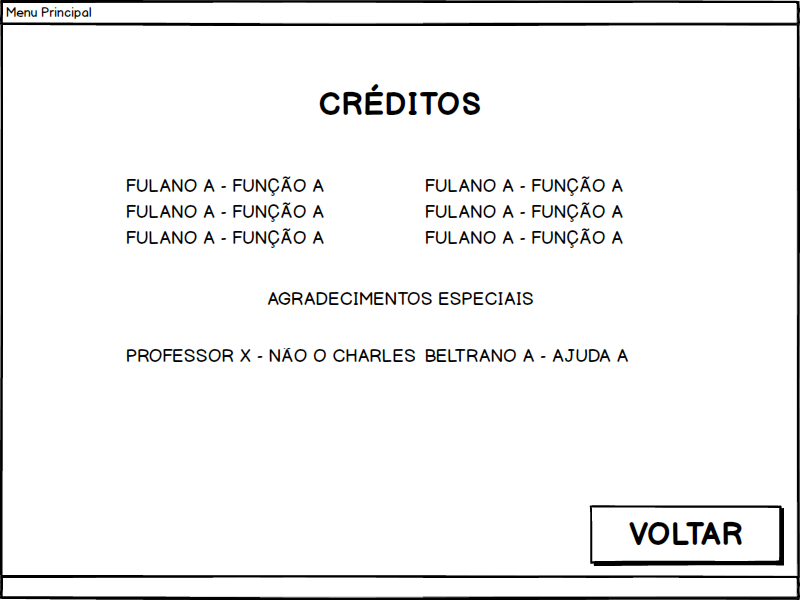
\includegraphics[keepaspectratio=true,scale=0.35]{images/CREDITOS.png}
\end{figure}

\begin{figure}[!h]
    \label{pause}
    \centering
    \caption{Tela de pause}
    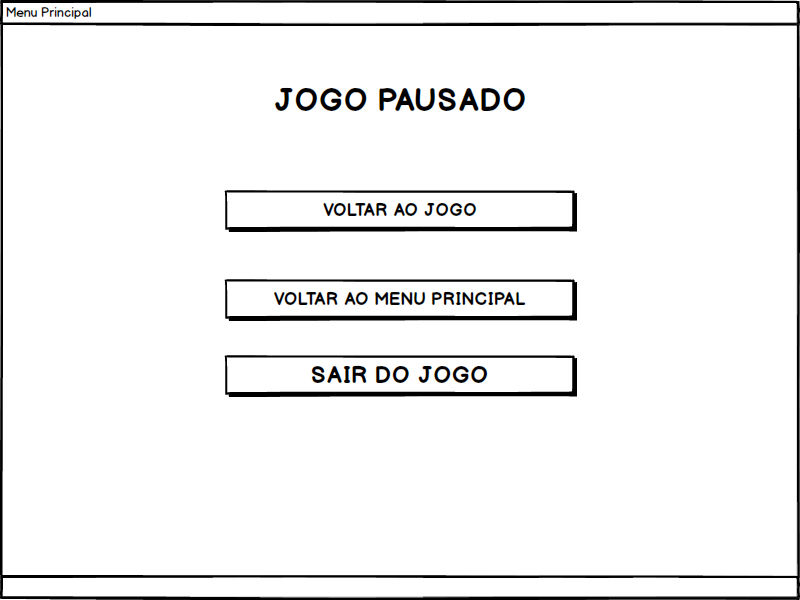
\includegraphics[keepaspectratio=true,scale=0.35]{images/PAUSE.png}
\end{figure}

\break

\section{Câmera e HUD}
A câmera do jogo é fixa e vista de um ângulo superior inclinado, mais conhecido como \lq\lq visão de pássaro\rq\rq. 

No canto superior esquerdo será apresentado as três barras de dados fundamentais do jogo na seguinte ordem: barra de vida, barra de resistência (stamina) e de sanidade. As barras estão alinhadas a uma imagem do rosto do player que irá variar de acordo com o nível da barra da sanidade.

No canto inferior esquerdo será apresentado os botões de ação do personagem que demonstram os itens que o player poderá utilizar, tanto para ataque quanto para se curar.

\begin{figure}[!h]
    \label{hud}
    \centering
    \caption{Câmera do HUD}
    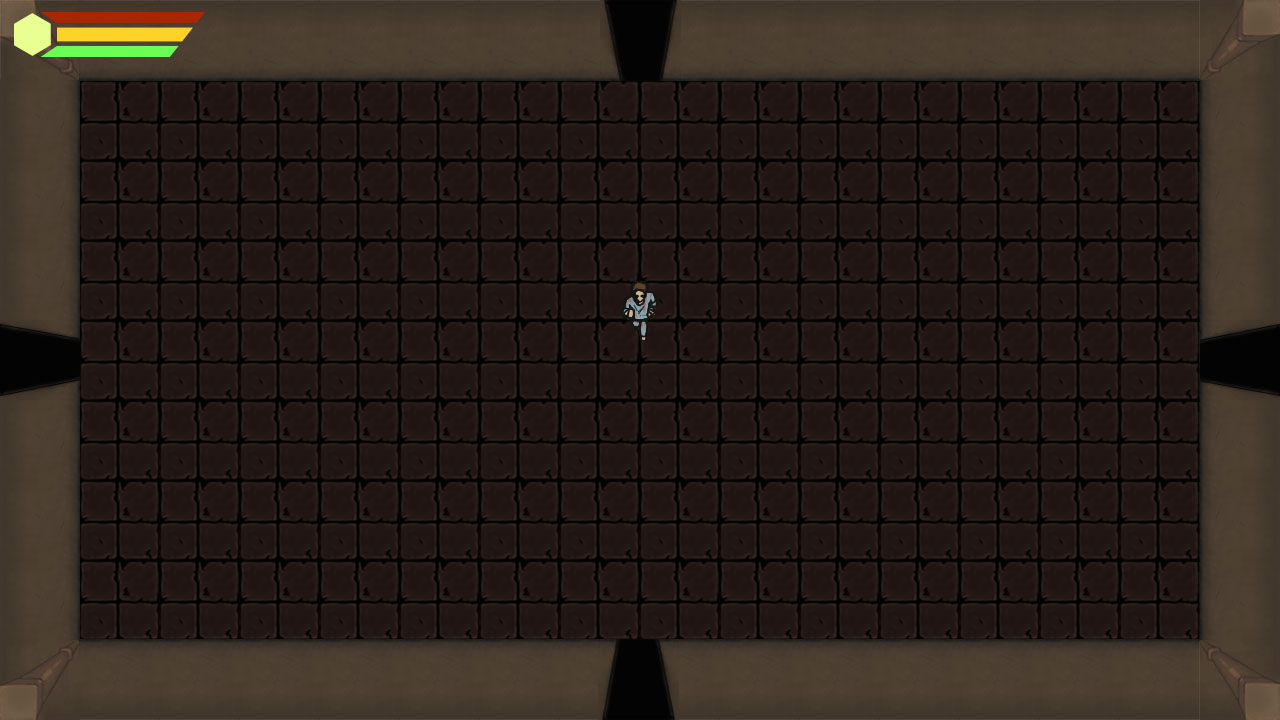
\includegraphics[keepaspectratio=true,scale=0.35]{images/HUD.jpg}
\end{figure}

\section{\label{ctrl} Controles}
O jogador poderá usar como forma de controle para o jogo o teclado do computador ou ainda controles para computadores, mais conhecidos como joysticks. A tabela presente nessa seção apresenta as devidas funcionalidades de ambas as opções dentro do jogo.

\begin{longtable}{|c|c|}
\caption{Controles do jogo}
\\
\hline
\multicolumn{2}{|c|}{Lista de comandos do jogo}
\\
\hline

\includegraphics[scale=0.3]{images/360_Dpad.png}

\includegraphics[scale=0.3]{images/kW.png} 

\includegraphics[scale=0.3]{images/kA.png}

\includegraphics[scale=0.3]{images/kS.png}

\includegraphics[scale=0.3]{images/kD.png}
& Movimentar o personagem na tela
\\
\hline

\includegraphics[scale=0.3]{images/360_RT.png}

\includegraphics[scale=0.3]{images/kShift.png}
 & Correr (na direção selecionada)
\\
\hline

\includegraphics[scale=0.3]{images/360_RB.png}

\includegraphics[scale=0.3]{images/kAlt.png}
& Rolar (na direção selecionada) 
\\
\hline

\includegraphics[scale=0.3]{images/360_LB.png}

\includegraphics[scale=0.3]{images/kCtrl.png}
& Agachar e andar agachado (pressionando algum botão direcional)
\\
\hline

\includegraphics[scale=0.3]{images/360_LT.png}

\includegraphics[scale=0.3]{images/kL.png}
& Ataque com arma secundária
\\
\hline

\includegraphics[scale=0.3]{images/360_A.png}

\includegraphics[scale=0.3]{images/kJ.png}
& Ataque principal (No menu: selecionar opção)
\\
\hline

\includegraphics[scale=0.3]{images/360_B.png}

\includegraphics[scale=0.3]{images/kK.png}
& Interagir com itens (No menu: negar opção)
\\
\hline

\includegraphics[scale=0.3]{images/360_X.png}

\includegraphics[scale=0.3]{images/kQ.png}
& Usar item 
\\
\hline

\includegraphics[scale=0.3]{images/360_Y.png}

\includegraphics[scale=0.3]{images/kE.png}
& Abre a porta especial (ao possuir a chave) 
\\
\hline

\includegraphics[scale=0.3]{images/360_Start.png}

\includegraphics[scale=0.3]{images/kP.png}
& Pausar jogo (acessa o menu de pausa)
\\
\hline
\end{longtable}

